\chapstart
\section{XÂY DỰNG ỨNG DỤNG VÀ THIẾT KẾ KIẾN TRÚC}
\subsection{Tổng quan kiến trúc Java + XML, MVVM + Repository + Model}
BroomSharing lựa chọn định hướng tổ chức ứng dụng thành các thành phần giao diện, trạng thái màn hình và truy cập dữ liệu. Định hướng này phù hợp với các khuyến nghị về phân tầng giao diện, dữ liệu và quản lý trạng thái của \textcite{android_views,android_data,android_viewmodel}.

\textbf{View} gồm các tệp XML, Activity/Fragment và Adapter, chịu trách nhiệm hiển thị danh sách, biểu mẫu, thông báo và tiếp nhận sự kiện người dùng. \textbf{ViewModel} nhận hành động từ View, xử lý trạng thái phục vụ giao diện, yêu cầu dữ liệu và cung cấp dữ liệu có thể quan sát. \textbf{Repository} cung cấp các thao tác làm việc với không gian, người dùng và booking, che giấu chi tiết gọi Firestore. \textbf{Model} gồm các lớp Java biểu diễn dữ liệu nghiệp vụ của ứng dụng.

\begin{figure}[H]\centering
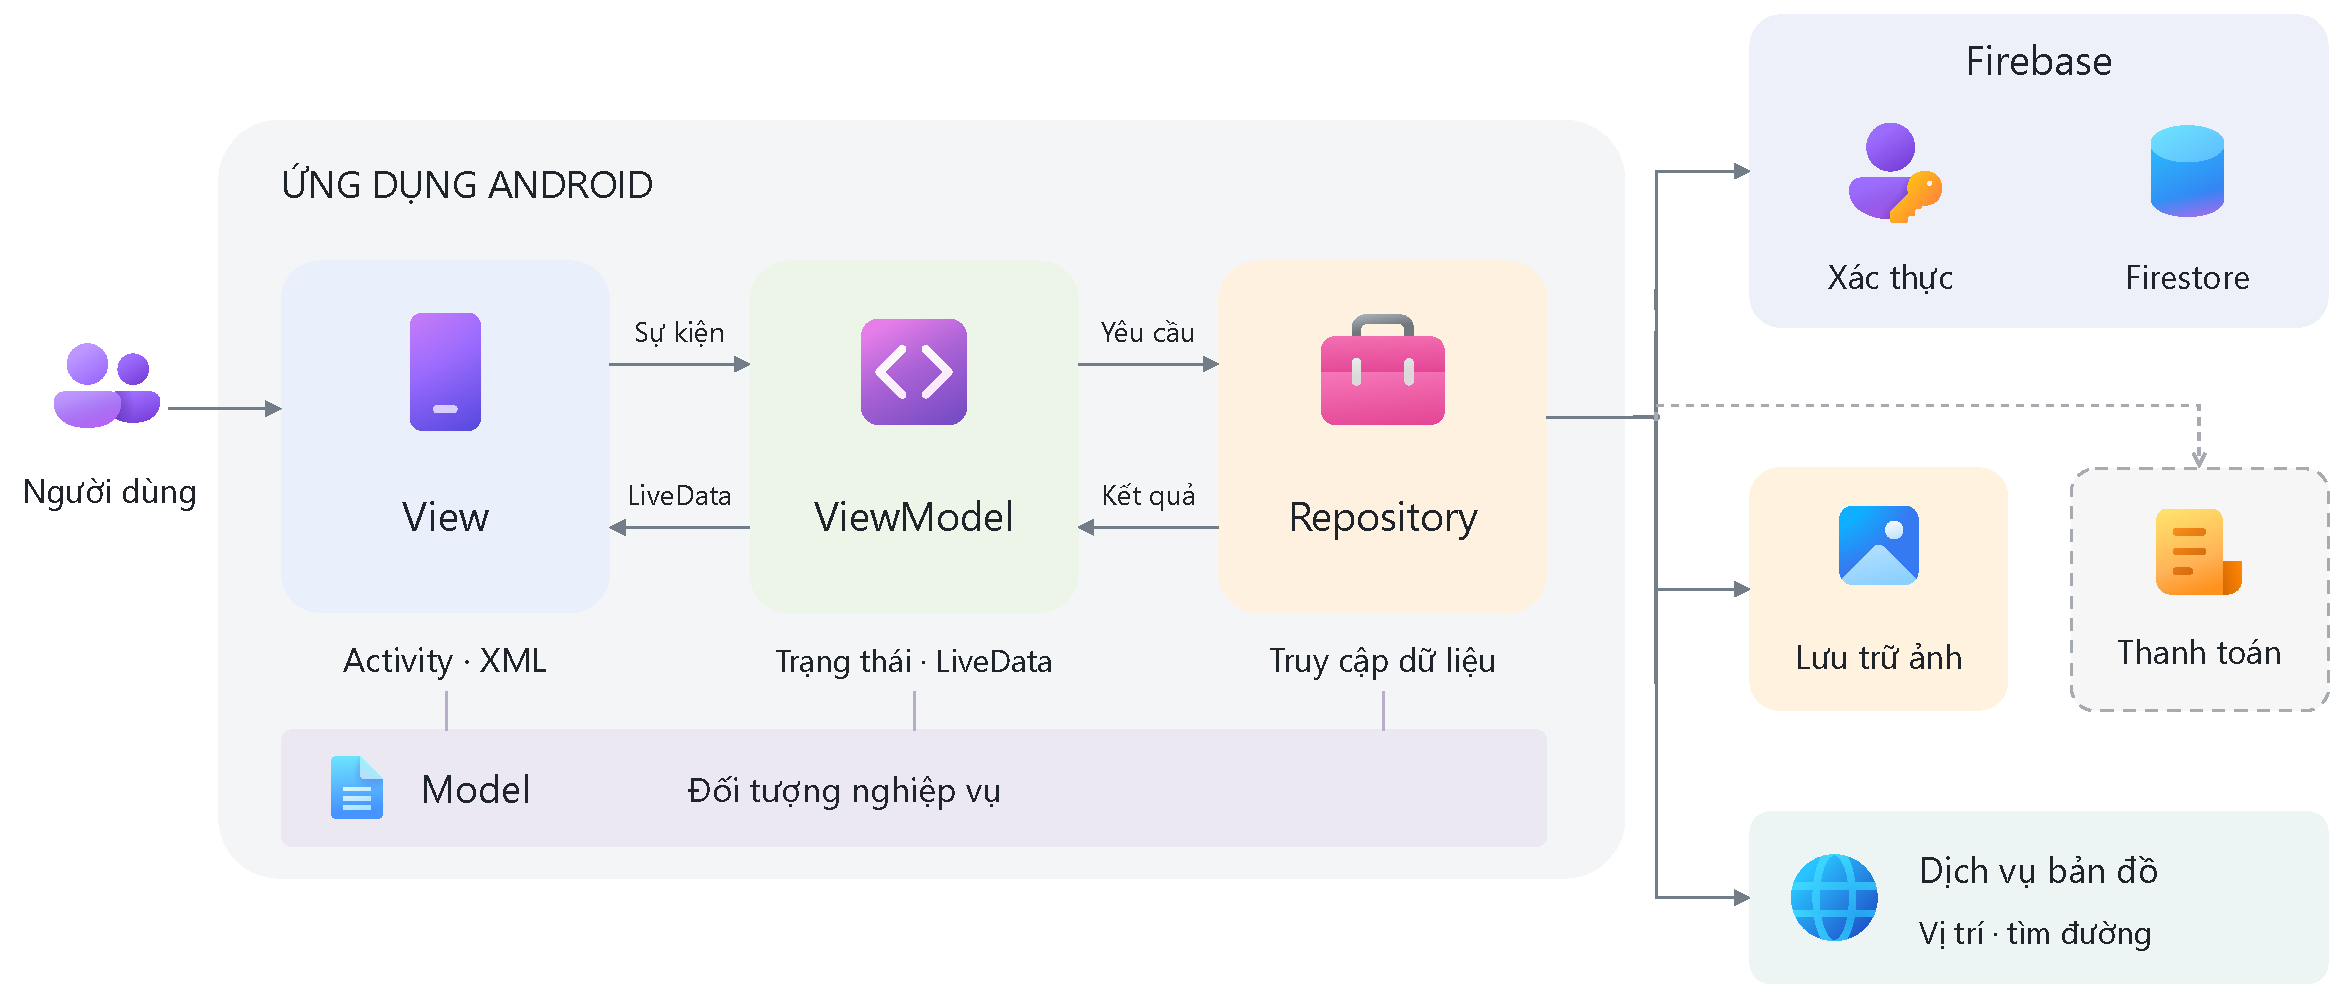
\includegraphics[width=\textwidth]{chapter5/application-architecture.pdf}
\caption{Kiến trúc tổng quan của ứng dụng BroomSharing}\label{fig:mvvm}
\end{figure}

Mũi tên từ View đến ViewModel biểu diễn lời gọi phương thức xử lý tương tác; chiều ngược lại biểu diễn dữ liệu trạng thái để View quan sát. ViewModel giao tiếp với Repository, không cần phụ thuộc vào API Firestore. Model được các thành phần sử dụng để biểu diễn dữ liệu nghiệp vụ. Nhánh thanh toán dùng nét đứt để thể hiện phần tích hợp dự kiến, chưa xác định nhà cung cấp.

\subsection{Cấu trúc thư mục đề xuất}
\begin{table}[H]\centering\small
\caption{Tổ chức gói mã nguồn Java + XML theo trách nhiệm}\label{tab:packages}
\begin{tabularx}{\textwidth}{@{}p{4.9cm}X@{}}\toprule
\textbf{Nhóm thư mục}&\textbf{Nhiệm vụ}\cr\midrule
\texttt{ui/} & Activity, Fragment, Adapter, ViewHolder và thành phần điều hướng.\\
\texttt{viewmodel/} & Ví dụ \texttt{SpaceViewModel}, \texttt{BookingViewModel}; cung cấp LiveData hoặc trạng thái tương ứng.\\
\texttt{repository/} & Ví dụ \texttt{SpaceRepository}, \texttt{BookingRepository}; đọc/ghi dữ liệu qua Firebase SDK.\\
\texttt{model/} & Các POJO \texttt{User}, \texttt{Space}, \texttt{Booking}, \texttt{Review} nếu cần.\\
\texttt{res/layout/} & XML cho Activity, Fragment, item danh sách và hộp thoại.\\
\texttt{res/drawable/}, \texttt{res/values/} & Ảnh, icon, màu, chuỗi và theme của ứng dụng.\\\bottomrule
\end{tabularx}\end{table}

\subsection{Kết nối với Firebase}
Ứng dụng Android cần được liên kết với dự án Firebase, cấu hình thư viện theo hướng dẫn chính thức và kiểm tra quyền đọc/ghi. Repository là nơi phù hợp để gọi \texttt{FirebaseFirestore} qua phương thức \texttt{getInstance()}, thực hiện truy vấn và ánh xạ tài liệu sang đối tượng Java. Hoạt động bất đồng bộ phải trả kết quả bằng callback/LiveData hoặc cơ chế tương đương; không thực hiện chờ mạng trên luồng giao diện \parencite{firebase_android,firebase_firestore}.

Đối với ảnh không gian, nên phân biệt tệp ảnh với bản ghi dữ liệu: tệp được quản lý bởi dịch vụ lưu trữ phù hợp; URL hoặc đường dẫn được tham chiếu trong \texttt{spaces}. Nếu phiên bản đồ án chỉ dùng ảnh tĩnh trong \texttt{drawable}, báo cáo phải mô tả đúng lựa chọn đó thay vì khẳng định có tải ảnh lên Storage.

\subsection{Minh họa luồng nghiệp vụ ``xem danh sách không gian''}
\begin{enumerate}[leftmargin=*]
\item Activity/Fragment tạo hoặc lấy ViewModel gắn với vòng đời giao diện.
\item View đăng ký quan sát danh sách không gian qua LiveData.
\item ViewModel gọi phương thức lấy danh sách ở SpaceRepository.
\item Repository truy vấn Firestore, ánh xạ document thành các đối tượng Space.
\item Khi có dữ liệu hoặc lỗi, ViewModel cập nhật trạng thái; View hiển thị thông tin qua RecyclerView hoặc trạng thái rỗng/lỗi tương ứng.
\end{enumerate}
Luồng này là \textbf{phương án tổ chức mã nguồn kiến trúc}; chưa phải bằng chứng rằng toàn bộ Activity hiện tại đã được refactor theo MVVM.

\subsection{Tích hợp bản đồ và ảnh trong kiến trúc}
Phần bản đồ và quản lý ảnh được bố trí như các dịch vụ tích hợp, không thay đổi nguyên tắc phân lớp chính của MVVM. Tab \textbf{Map} sử dụng \texttt{MapView} của MapLibre trong XML và Activity/Fragment Java để hiển thị bản đồ. Repository truy xuất danh sách không gian có tọa độ từ Firestore; lớp giao diện nhận dữ liệu đã được ViewModel cung cấp và đặt marker. Khi chọn tìm đường, thành phần tích hợp openrouteservice nhận điểm đi/đến, đọc GeoJSON và chuyển hình học tuyến để hiển thị trên MapLibre. MapTiler cung cấp style/tile và có thể hỗ trợ chuyển đổi địa chỉ thành tọa độ \parencite{maplibre_android,maptiler_geocoding,ors_directions}.

Ảnh không gian được chọn ở giao diện, tải lên Cloudinary theo cấu hình cho phép; sau khi thành công, ứng dụng cập nhật URL vào tài liệu \texttt{spaces} trên Firestore. Chỉ nên đưa vào báo cáo cuối kỳ các bước đã có mã nguồn và kết quả chạy. Việc gọi API mạng phải bất đồng bộ; không lưu khóa bí mật dịch vụ ở dạng hard-code trong ứng dụng \parencite{cloudinary_android}.

\begin{table}[H]\centering\small
\caption{Vai trò các công nghệ và luồng phụ trợ trong kiến trúc}\label{tab:services}
\begin{tabularx}{\textwidth}{@{}p{4.0cm}X@{}}\toprule
\textbf{Thành phần}&\textbf{Trách nhiệm trong thiết kế}\\\midrule
MapLibre Native & Thành phần Android View để hiển thị bản đồ, marker và đường đi.\\
MapTiler & Cung cấp dữ liệu bản đồ và geocoding theo API key.\\
openrouteservice & Trả dữ liệu tuyến đường giữa các tọa độ, ví dụ GeoJSON.\\
Android Location & Lấy tọa độ của thiết bị khi đã có quyền phù hợp.\\
Cloudinary & Upload và lưu trữ tệp ảnh, trả URL để ghi vào Firestore.\\
Cloud Firestore & Lưu các bản ghi nghiệp vụ, thuộc tính tọa độ và URL ảnh.\\\bottomrule
\end{tabularx}\end{table}

\subsection{Các màn hình và mức độ hoàn thiện}
Màn hình khám phá, chi tiết, bản đồ, đặt chỗ, đăng không gian, lịch sử booking, tin nhắn, hồ sơ và quản trị đã được thảo luận ở giai đoạn thiết kế UI. Để ghi nhận là \textit{đã xây dựng}, từng màn hình cần có tệp layout/Activity thật, ảnh chụp và một mục kiểm thử. Giai đoạn thiết kế có thể chấp nhận việc một số màn hình chỉ có bố cục XML hoặc dữ liệu mẫu; giai đoạn báo cáo thực thi phải mô tả khác biệt này rõ ràng.
